\section{Resultados e discussões}

\subsection{Viscosímetro de Stokes}\label{sec:viscStokes}
% Magina, aqui
    A partir dos dados coletados pelos grupos da turma foi montada uma tabela, posteriormente então repassada às equipes e recebeu alguns ajustes. Segue abaixo:

\begin{table}[H]
    \centering
    \caption{Valores medidos pelos grupos}
    \resizebox{\textwidth}{!}{%
    \begin{tabular}{l l l l l l l l}
        \hline
        \textbf{Medida} & \textbf{JOAQUIM} & \textbf{LARISSA} & \textbf{MICAEL} &
        \textbf{GIOVANA} & \textbf{LUIZA} & \textbf{JOSÉ} & \textbf{Média}  \\ \hline
        DENSIDADE (g/cm\(^3\)) & ?? & 0,879 & 0,88 & 0,88 & 0,88 & 0,883 & 0,8804  \\ 
        ~ & ~ & ~ & ~ & ~ & ~ & ~ &   \\ 
        diâmetro da esfera 1 (mm) & 1,998 & 2,752 & 3,252 & 3,948 & 4,754 & 5,494 &   \\ 
        d2 & 1,991 & 2,768 & 3,167 & 3,959 & 4,753 & 5,497 &   \\ 
        d3 & 1,983 & 2,765 & 3,184 & 3,958 & 4,754 & 5,5 &   \\ 
        d4 & 1,991 & 2,768 & 3,186 & 3,934 & 4,754 & 5,496 &   \\ 
        dMED & 1,99075 & 2,76325 & 3,19725 & 3,94975 & 4,75375 & 5,49675 &   \\ 
        raioMED & 0,995375 & 1,381625 & 1,598625 & 1,974875 & 2,376875 & 2,748375 &   \\ 
        raioMED² (mm²) & 0,990771391 & 1,908887641 & 2,555601891 & 3,900131266 & 5,649534766 & 7,553565141 &   \\ 
        ~ & ~ & ~ & ~ & ~ & ~ & ~ &   \\ 
        tempo de queda 1 (s) & 8,19 & 4,32 & 3,34 & 2,28 & 1,66 & 1,41 &   \\ 
        t2 & 8,4 & 4,34 & 3,56 & 2,42 & 1,78 & 1,34 &   \\ 
        t3 & 8,31 & 4,38 & 3,66 & 2,53 & 1,72 & 1,4 &   \\ 
        t4 & 4,44 & 4,4 & 3,35 & 2,31 & 1,78 & 1,5 &   \\ 
        ~ & ~ & ~ & ~ & ~ & ~ & ~ &   \\ 
        Diâmetro do tubo 1 (mm) & 4,932 & 4,88 & 4,7 & 4,86 & 4,8 & 4,844 &   \\ 
        D2 & 4,84 & 4,899 & ?? & 4,84 & 4,9 & 4,944 &   \\ 
        D3 & 4,842 & 4,864 & ?? & 4,88 & 4,903 & 4,84 &   \\ 
        D4 & 4,936 & 4,864 & ?? & 4,94 & 4,878 & ?? &   \\ 
        DMED & 4,8875 & 4,87675 & 4,7 & 4,88 & 4,87025 & 4,876 & 4,8781*  \\ 
        ~ & ~ & ~ & ~ & ~ & ~ & ~ &   \\ 
        Altura percorrida (cm) & 30 & 30 & 30 & 30 & 30 & 30 & 30  \\ 
        VelocidadeMED (cm/s) & 4,08997955 & 6,880733945 & 8,626887132 & 12,57861635 & 17,29106628 & 21,23893805 &   \\ \hline
    \end{tabular}
    } %fecha o resize
    \subcaption*{Nota: a média marcada com * desconsidera o valor do grupo ``Micael", por este ter coletado apenas uma medida, sendo muito discrepante em relação às demais.}
\end{table}
Os fatores que foram medidos diferentemente pelos grupos foram os diâmetros das esferas e os tempos e velocidades com que caíram. Percebeu-se um padrão de maior a velocidade quanto maior o diâmetro. Para compreender melhor como o diâmetro, e analogamente o raio, das esferas afeta sua descida, foi feito um gráfico das velocidades em função do raio ao quadrado, como segue:
\begin{figure}[H]
    \centering
    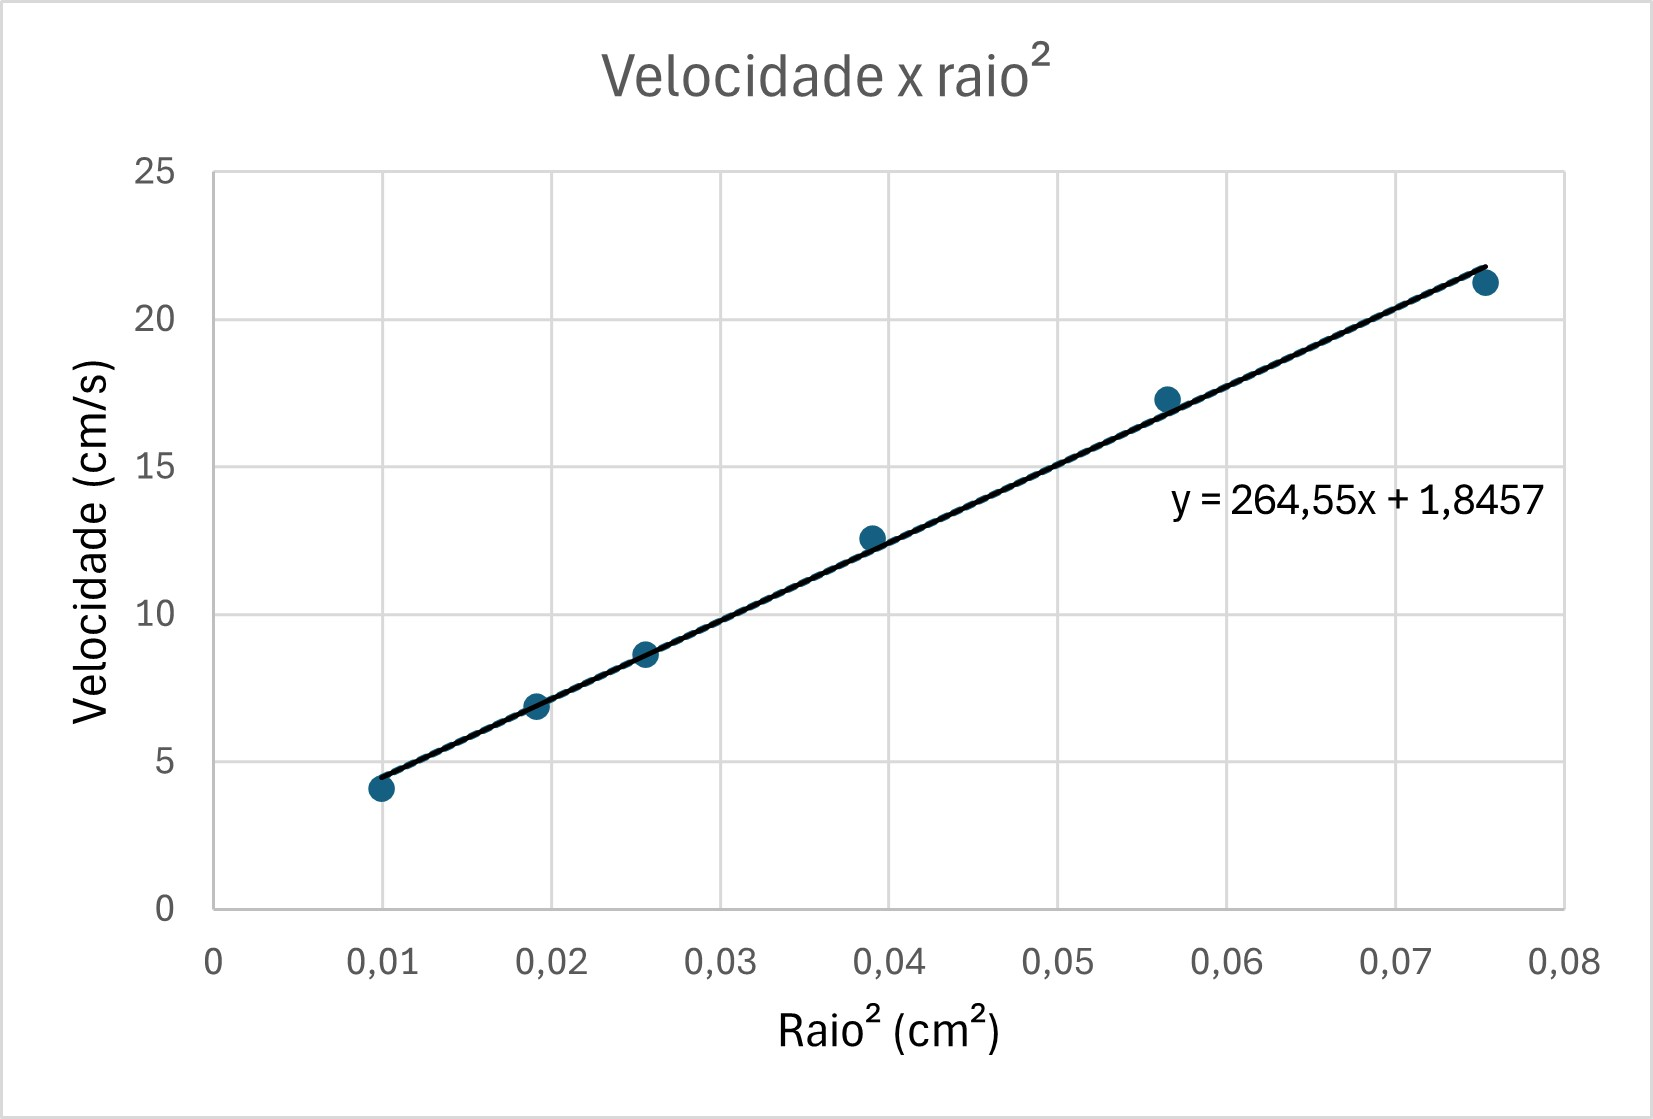
\includegraphics[width=0.6\textwidth]{fig/GraficoViscosimetroV2.jpg}
    \caption{Gráfico da velocidade em função do raio ao quadrado}
    \label{fig:grafVisc}
\end{figure}
Pela análise do gráfico pode-se notar que a velocidade comporta-se se forma quase linear com o raio ao quadrado, logo uma fórmula que relacione as duas deve ter o raio ao quadrado, como ocorre na lei de Stokes para a velocidade limite:
\begin{align*}
    v\text{limite} =\frac{2g}{9\eta}(\rho \text{esf}- \rho \text{fluido})r^2
\end{align*}
Para uma maior precisão, deve-se converter a velocidade medida para a velocidade em um tubo de diâmetro infinito, pela seguinte fórmula:
\begin{align*}
    v \infty = \left(1 + \frac{9r}{2D} + \left(\frac{9r}{2D}\right)^2\right) \cdot v 
\end{align*}
Com isso, obtem-se o seguinte gráfico, fornecido pelos orientadores do trabalho:
\begin{figure}[H]
    \centering
    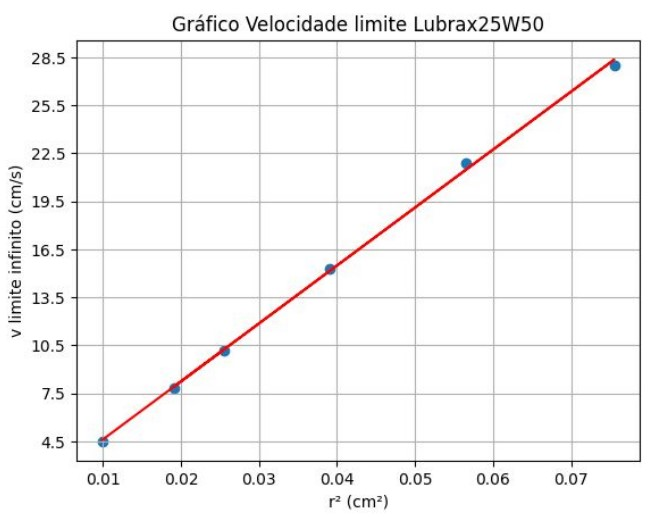
\includegraphics[width=0.6\textwidth]{fig/GraficoOrientadores.jpg}
    \caption{Gráfico da velocidade limite em tubo infinito pelo raio ao quadrado}
    \label{fig:grafVisc2}
\end{figure}
Tendo em vista a esfera caindo pelo viscosímetro, tem-se o seguinte diagrama de forças sobre ela\footnote{\url{https://edisciplinas.usp.br/pluginfile.php/8929729/mod_resource/content/0/Aula\%2011\%20-\%2007_04_25.pdf}}:
\begin{figure}[H]
    \centering
    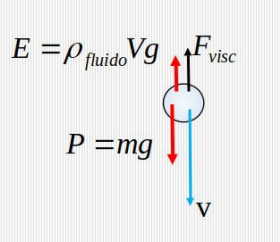
\includegraphics[width=0.3\textwidth]{fig/DiagramaDeForcas.png}
    \caption{Diagrama de forças. Fonte: slides fornecidos pelos orientadores.}
    \label{fig:grafVisc}
\end{figure}
Podemos então calcular o coeficiente de viscosidade \(\eta\) a partir da lei de Stokes e o empuxo pelo Princípio de Arquimedes. Ao igualar a força peso ao empuxo mais a viscosidade, uma vez que a esfera desce à velocidade constante, as forças se compensam. Considere \(\rho f\) a densidade do fluído e \(\rho e\) a densidade da esfera, assim:
\begin{align*}
    P = E + F\text{visc}
    \\
    mg = V \rho f g + 6 \pi \eta r v
    \\
    V \rho e g =  V \rho f g + 6 \pi \eta r v
    \\
    \eta = \frac{V \rho e g - V \rho f g}{6 \pi r v}
    \\
    \eta = \frac{4 \pi r^3}{3}\cdot \frac{ g (\rho e - \rho f)}{ 6 \pi r v}
    \\
    \eta = \frac{2 r^2 g (\rho e - \rho f)}{ 9 v}
\end{align*}
Além disso, se utilizarmos o coeficiente angular do gráfico da
\cref{fig:grafVisc2}, \(k\), podemos reescrever a fórmula da seguinte maneira:
\begin{align*}
    \eta = \frac{2 g (\rho e - \rho f)}{ 9 k}
\end{align*}
Com isso, foram calculados pelos orientadores os seguintes valores de viscosidade:
\begin{table}[H]
    \centering
    \caption{Coeficientes de viscosidade \(\eta\)}
    \begin{tabular}{|l|l|}
        \hline
        Viscosidade (poise) & 4,19  \\ \hline
        Viscosidade (cP) & 419 \\ \hline
        \(\sigma\) viscosidade (cP) & 31  \\ \hline
        Viscosidade cinética (cSt) & 476   \\ \hline
        \(\sigma\) viscosidade cinética (cSt) & 35  \\ \hline
        Valor de referência tabelado (cSt) & 438  \\ \hline
    \end{tabular}
\end{table}
Todavia, é possível notar que o valor obtido (\(476 \pm 35\) cSt) diverge do esperado (438 cSt), inclusive estando fora da margem de incerteza calculada. O erro percentual encontra-se em 9\%. Uma explicação para tal divergência é a baixa precisão das medidas, como o tempo de descida dependente do tempo de reação humano (cerca de 200ms)\footnote{\url{https://en.wikipedia.org/wiki/Mental_chronometry}} e da observação visual se a esfera em movimento havia entrado e saído da região desejada do líquido. Já outra explicação é pela alta influência temperatura, pois pela tabela fornecida a viscosidade cinética do líquido varia de 465,83 a 412,39 cSt no intervalo de 24 a 26\(^\circ\)C.


\subsection{Fenômeno de planagem}
\subsubsection{Asa de um avião}
% Magina, aqui
    Ao ligar o ventilador a asa de isopor subia no fio, até uma altura próxima à do
    centro da hélice e lá permanecia estável com pequenos tremores. Caso se forçasse
    a asa para baixo ela apresentava resistência e, assim que solta, voltava à
    posição elevada. Já se um integrante levantasse a asa e a soltasse, ela caía até
    a mesma posição e lá permanecia.

    Tendo em vista que as principais forças atuantes eram o peso da asa e as
    resultantes da interação do objeto com o ar, como o empuxo, pode-se concluir que
    com o acionamento do ventilador a pressão do ar embaixo da asa tornava-se maior
    que aquela em cima, fazendo uma força ascendente por conta do empuxo resultante.
    O grupo aponta que essa diferença de pressão ocorre, ao menos majoritariamente,
    por conta da forma da asa, que afeta como o ar passará por ela.

    Já ao ultrapassar a altura de estabilidade essa força ascendente não era mais
    suficiente para vencer o peso, de forma que ela descia. Possivelmente isso
    ocorre porque ao passar da altura do eixo do ventilador o vento ficaria
    proporcionalmente mais rápido embaixo, o que reduz a pressão nessa região pelo
    efeito Venturi (maior velocidade do fluído abaixa sua pressão). Com isso, ela
    permanece estável no ponto em que a força peso e o empuxo do ar causado pela
    diferença de pressão se equilibram, sem descer pois isso aumentaria a diferença
    de pressão e consequentemente o empuxo, e sem subir porque a diferença reduziria
    juntamente ao empuxo. 

\subsubsection{Tubo de Pitot}
    A relação entre as medidas relativas de pressão e os pontos medidos foi
    sintetizada na \cref{erapraserumquadro-sequiserarrumevc}.
    %Aqui deveria ser um quadro, porém não tenho como criar essa estrutura agora
    %sem o risco de errar a numeração. Em prol de uma boa numeração, não irei
    %arrumar isso. Aquele que se sentir disposto pode fazê-lo.
    \begin{table}[H]
    \caption{Medidas relativas de pressão observadas}\label{erapraserumquadro-sequiserarrumevc}
    \begin{center}
    \begin{tabular}{c c c}
    \hline
    Tubo & Local & Pressão Relativa à Pressão Atmosférica \\
    \hline
    1    & Parte frontal da asa & Parcialmente positiva\\
    2    & Parte superior da asa & Negativa\\
    3    & Parte inferior da asa & Parcialmente negativa\\
    \hline
    \end{tabular}
    \end{center}
    \end{table}
    Assim, fica evidente a relação dessas medidas com o fenômeno de planagem: a
    diferença de pressões entre a parte inferior e a superior da asa geram uma
    força de pressão direcionada para cima (região com menor pressão). Além
    disso, a pressão parcialmente positiva na parte frontal da asa se relaciona
    com o ponto de estagnação, onde toda a energia cinética do fluido é
    convertida em pressão, que foi estudada no tubo de Pitot.

\subsection{Tubos com esfera}
\subsubsection{Análise qualitativa dos fluidos}
% Luan, aqui
    Após analisar os tubos fechados, observou-se que em um dos tubos a esfera se
    moveu mais lentamente que no outro. Essa diferença pode ser atribuída a
    diferença de viscosidade dos fluidos, tendo em vista que uma força de
    resistência viscosa maior seria responsável por uma velocidade terminal
    menor da esfera. Em relação ao fluido do viscosímetro, veja
    a \cref{sec:viscStokes}, onde foi realizada uma discussão mais
    detalhada da viscosidade e o movimento das esferas nesse meio.

\subsubsection{Análise quantitativa das velocidades}
% Luan, aqui
% Aguardando os vídeos
    As sessões dos tubos tinham distância média de
    \qty{5.00\pm0.05}{\centi\meter} e ambos os tubos tinham um total de 12
    seções. Com a análise dos vídeos gravados durante a experimentação, obtemos
    a \cref{tab:tubos}:
    \begin{table}[H]
    \caption{Dados cinemático obtidos por uso do
    Tracker\textsuperscript{\textcopyright}}\label{tab:tubos}
    \begin{center}
    \begin{tabular}{c c c c c}
    \hline
    Tubo & \( \Delta x \) & \( \Delta t \) & \( v_m \) & Tempo estimado para o
    percurso \\
    \hline
    Tubo 1 & \qty{5.00\pm0.05}{\centi\meter} & \qty{15.648}{\second} &
    \qty{0.320}{\centi\meter\per\second} & \qty{188}{\second} \\
    Tubo 2 & \qty{5.00\pm0.05}{\centi\meter} & \qty{1.635}{\second} &
    \qty{3.06}{\centi\meter\per\second} & \qty{19.6}{\second} \\
    \hline
    \end{tabular}
    \end{center}
    \end{table}
    Note que os algarismos significativos e os erros associados a cada medida
    foram atribuídos conforme a ferramenta de medida utilizada.  Além disso,
    observe a diferença entre os tempos estimados, o Tubo 2 possui uma
    estimativa cerca de 10 vezes menor que o Tubo 1. Como discutimos
    anteriormente, essa diferença está fundamentalmente atrelada às diferenças
    de viscosidade dos fluidos, tendo em vista que os outros parâmetros da
    experimentação se mantiveram constantes. 

